\documentclass{article}

% Style file (FinalReport.sty) is the verbatim NeurIPS 2026 style, renamed.
\usepackage[preprint]{FinalReport}

\usepackage[utf8]{inputenc} % allow utf-8 input
\usepackage[T1]{fontenc}    % use 8-bit T1 fonts
\usepackage{hyperref}       % hyperlinks
\usepackage{url}            % simple URL typesetting
\usepackage{booktabs}       % professional-quality tables
\usepackage{amsmath}        % \text, \dfrac, etc.
\usepackage{amsfonts}       % blackboard math symbols
\usepackage{nicefrac}       % compact symbols for 1/2, etc.
\usepackage{microtype}      % microtypography
\usepackage{xcolor}         % colors
\usepackage{graphicx}       % figures
\usepackage{placeins}       % \FloatBarrier

\title{Modeling for Acquisition Entrepreneurship:\\
       AutoResearch Deployed on U.S.\ Midwest IT MSPs}

\author{Yutong Wen
\\ Northwestern University
\\ \texttt{yutongwen2026@u.northwestern.edu}}

\begin{document}

\maketitle

\begin{abstract}
We construct an AutoResearch agent loop that automates the identification of high-quality
acquisition targets among U.S.\ Midwest IT Managed Service Providers (MSPs). Across 20
controlled experiments, two \emph{continuous structural facts} --- a quadratic
\emph{Succession Curve} over founder tenure (\texttt{tenure\_sq}) and a \emph{Stagnation
Premium} on revenue-per-employee (\texttt{rev\_per\_emp}) --- account for nearly all
generalizable signal, while five sparse NLP-feature attempts uniformly fail the
$\geq 16\%$ tag-rate sparsity floor implied by our $N{=}62$ training set. A SHA-256-locked
Worker/Judge architecture and an explicit Decoupled Isolation Rule prevent two would-be
promotion errors --- notably the Exp\_016 \emph{compliance}-keyword artifact, caught by
a targeted ablation audit. The champion model achieves a single-pass holdout RMSE of
\textbf{1.5119} on 28 unseen firms (vs.\ a 1.3955 cross-validation RMSE on training),
comfortably below the project's pre-declared $<2.0$ success ceiling. We discuss why
agent-driven loops are exceptionally vulnerable to small-sample text artifacts and why
human adversarial audits remain irreplaceable.
\end{abstract}

\section{Introduction}
\label{sec:intro}
In an Acquisition Entrepreneurship (``Search Fund'') model, an entrepreneur raises capital
to buy and operate a single small business from a retiring founder. The bottleneck is
\emph{sourcing}: identifying unlisted firms that simultaneously satisfy the textbook
``stable but stagnant'' rubric --- deep founder tenure, recurring revenue, modest scale,
operational slack --- takes hundreds of analyst hours. We formalize the sourcing question
as supervised ordinal regression: given a firm's firmographic profile and public web copy,
predict an investment-grade score from $1.0$--$10.0$ in strict $0.5$-point increments.
Training set: 62 manually labeled Midwest IT MSPs. Test set: 28 unseen firms scored
exactly once.

\textbf{Contributions.}
(i)~An end-to-end AutoResearch agent loop with a tamper-evident Worker/Judge split and
protocols that empirically prevent agent self-deception (\S\ref{sec:method}).
(ii)~Across 20 controlled runs we identify two robust signals and one decisive failure
mode --- a small-$N$ keyword artifact detected by targeted ablation
(\S\ref{sec:trajectory}, Fig.~\ref{fig:eda}--\ref{fig:trajectory}).
(iii)~A single-pass test RMSE that comfortably beats the $<2.0$ ceiling
(\S\ref{sec:results}), plus a frank treatment of the limits of the loop
(\S\ref{sec:limitations}).

\section{Method}
\label{sec:method}

\paragraph{Worker/Judge with a one-way valve.}
The agent may only modify \texttt{model.py} (the Worker: feature engineering, regressor,
post-processing). The evaluation file \texttt{eval/prepare.py} (the Judge: split, metric,
log-append) is frozen by SHA-256 \texttt{8f7aa10f25b1...} and verified before every Worker
run; the orchestrator \texttt{run\_experiment.py} aborts if the hash drifts.

\paragraph{Decoupled Isolation Rule.}
Each Controlled Experiment begins with a clean
\texttt{cp logs/Snapshot\_model\_Exp\_009.py model.py} revert; exactly one variable changes
per run, tested at the baseline regularization $\alpha{=}1.0$. Hyperparameter tuning is
deferred to a separate follow-up run only if a positive signal is observed at the
baseline. This rule was codified after the Exp\_012 confound, in which a bundled
feature-plus-tuning run shifted $\alpha$ from $1$ to $10$ and erased the load-bearing
\texttt{tenure\_sq} coefficient.

\paragraph{The 5$\times$ Alpha Guardrail.}
Any \texttt{GridSearchCV} that selects an $\alpha$ more than five times above or below the
baseline is automatically flagged for review. Empirically this fires when a new feature
introduces collinearity that the optimizer ``solves'' via over-shrinkage.

\paragraph{Five research axes.}
We organize the 20 runs into five hypothesis families (Table~\ref{tab:axes}):
\textbf{Demographics} (tenure, size, geography), \textbf{Operational Efficiency} (revenue
ratios, MRR keywords), \textbf{Ownership/Succession} (founder/acquisition detection),
\textbf{Competitive Moat} (regulated-industry verticals), and \textbf{Model Integrity}
(regularization, ensembling, post-processing).

\begin{table}[h]
  \caption{Five research axes after 20 controlled experiments. Two ``Core'' axes carry
  the entire generalizable signal; one axis (Moat) was disqualified by audit; the
  Ownership axis is real-but-sparse; Model Integrity is the empirical motivation for the
  isolation protocols.}
  \label{tab:axes}
  \centering\small
  \begin{tabular}{@{}lllp{2.05in}@{}}
    \toprule
    \textbf{Axis} & \textbf{Key feature} & \textbf{Status} & \textbf{Impact} \\
    \midrule
    Demographics      & \texttt{tenure\_sq}          & Core         & Succession bell curve; load-bearing in all healthy runs. \\
    Operational       & \texttt{rev\_per\_emp}       & \textbf{Champion} & Stagnation Premium; Exp\_009 baseline, RMSE 1.3955. \\
    Ownership         & \texttt{founder\_led} family & Exploratory  & 5 correctly-signed but sparse failures (3--11\% tags). \\
    Competitive Moat  & \texttt{has\_moat}           & Discarded    & Disqualified by Exp\_018 \emph{compliance}-keyword audit. \\
    Model Integrity   & Bagging / Interaction / HGBR & Discarded    & Ridge($\alpha{=}1.0$) is the right inductive bias at $N{=}62$. \\
    \bottomrule
  \end{tabular}
\end{table}

\section{Experimental Trajectory}
\label{sec:trajectory}

\paragraph{Demographics and Operational success (Exp\_002, Exp\_009).}
Exp\_002 introduced a 9-feature Ridge model with \texttt{tenure} and \texttt{tenure\_sq}
as the demographic core, cutting RMSE from 1.8460 (hand-coded boolean rules) to 1.5112 in
one step. Seven experiments later, Exp\_009 added a single structural feature
\texttt{rev\_per\_emp $=$ revenue/employees}, dropping RMSE to \textbf{1.3955} --- a
$-7.1\%$ improvement over the prior best. The Ridge coefficient on \texttt{rev\_per\_emp}
is $-0.66$ (standardized), and the bell-curve pair (\texttt{tenure}~$+0.66$,
\texttt{tenure\_sq}~$-0.31$) is preserved alongside it (Fig.~\ref{fig:eda}).

\paragraph{The text-feature wall (Exp\_013--Exp\_015, Exp\_020).}
Four binary NLP features for founder presence and prior acquisition produced
correctly-signed coefficients (all negative, ranging from $-0.11$ to $-0.36$) but
consistently failed RMSE. Their tag rates --- 6.5\%, 4.8\%, 11.3\%, 4.8\% --- fall below
the $\sim 16\%$ \emph{sparsity floor} we observe empirically at $N{=}62$: below that
density, the variance of fitting an additional Ridge coefficient exceeds the bias-reduction
the feature provides. The pattern is robust across the family.

\begin{figure}[t]
  \centering
  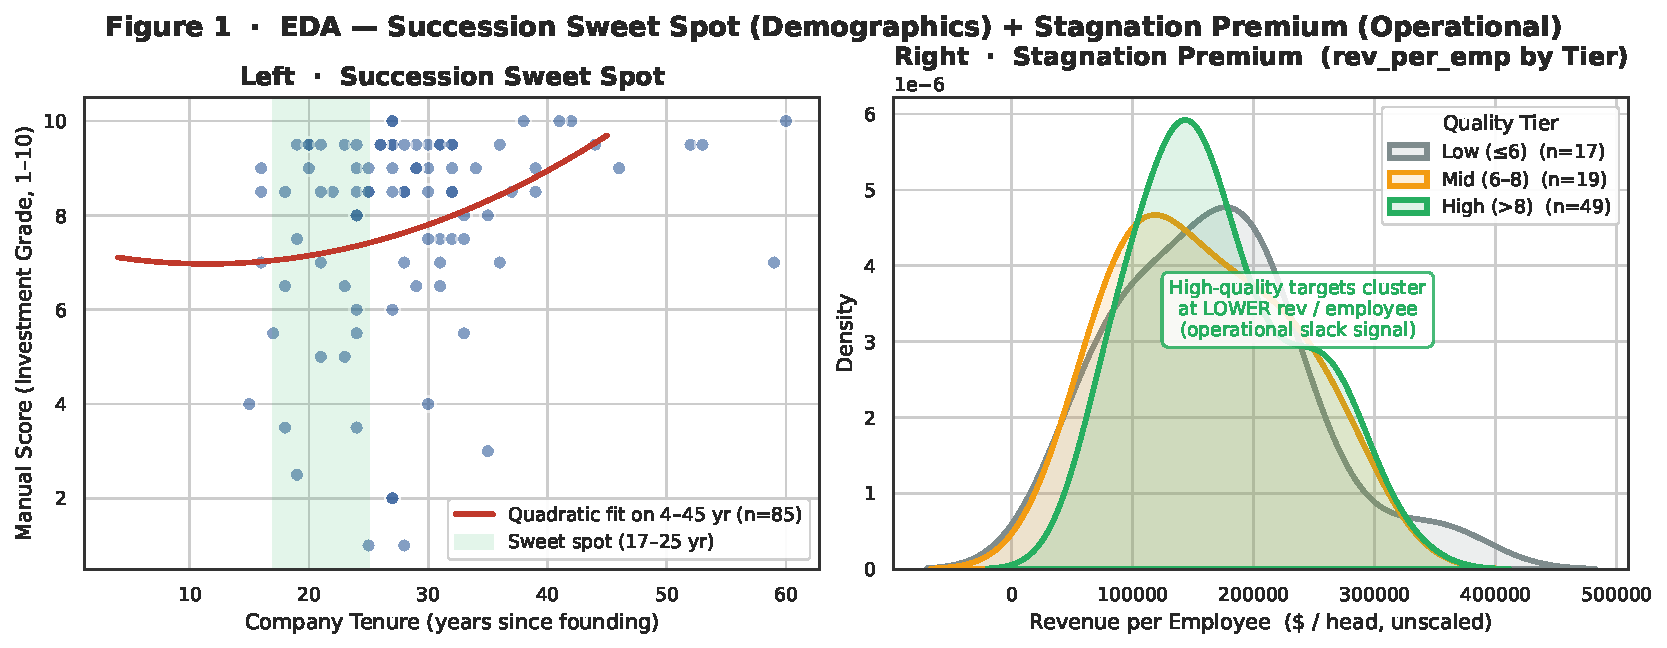
\includegraphics[width=0.92\linewidth]{plots/figure_1_eda.pdf}
  \caption{\textbf{Left:} Manual Score vs.\ company tenure on the 90 labeled firms, with a
  quadratic fit restricted to 4--45 years (where the search-fund thesis is well-posed); the
  fit peaks in the 17--25 year founder-retirement band.
  \textbf{Right:} KDE of revenue-per-employee, faceted by quality tier. High-quality
  targets (Score~$>$~8) cluster at \emph{lower} \texttt{rev\_per\_emp} --- the empirical
  content of the Stagnation Premium.}
  \label{fig:eda}
\end{figure}

\begin{figure}[t]
  \centering
  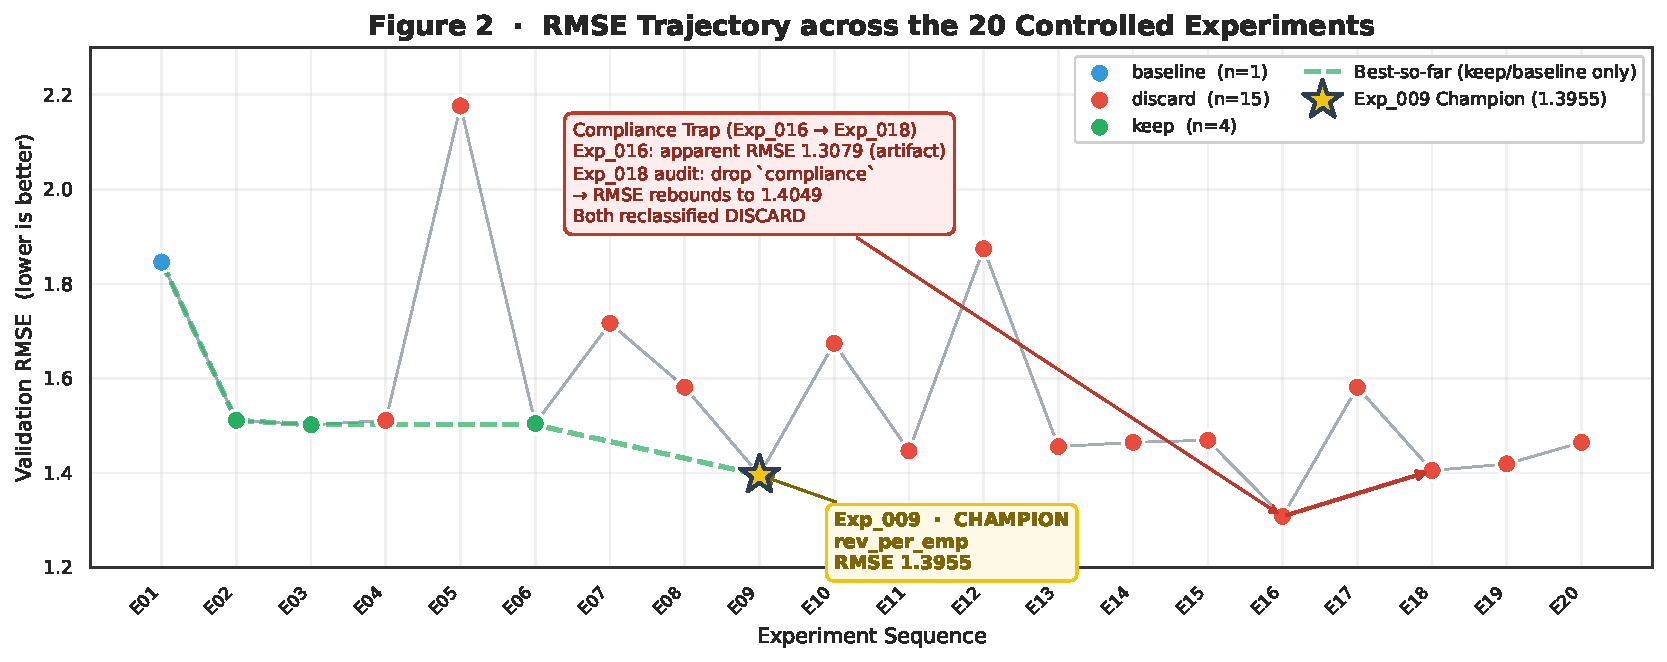
\includegraphics[width=0.92\linewidth]{plots/figure_2_trajectory.pdf}
  \caption{Validation RMSE across the 20 controlled experiments. The best-so-far envelope
  (dashed green) respects status, so the Exp\_016 \emph{compliance} artifact does not
  appear on the frontier. Yellow star = Exp\_009 champion (RMSE 1.3955). The red callout
  details the Exp\_016~$\to$~Exp\_018 compliance-trap-then-audit-rebound narrative central
  to \S\ref{sec:trajectory}.}
  \label{fig:trajectory}
\end{figure}
\FloatBarrier

\paragraph{The compliance trap (Exp\_016) and audit rebound (Exp\_018).}
Exp\_016 added a single binary \texttt{has\_moat} tagging firms whose Short Description
contained any of \{\emph{hipaa, dental, legal, law firm, manufacturing, pci, compliance,
regulated}\}; it produced an apparent new all-time best of RMSE \textbf{1.3079}. Three
red flags surfaced in the diagnostic: tag rate $88.7\%$; coefficient sign \emph{opposite}
the stated hypothesis ($-0.58$); and the \emph{compliance} keyword alone tagging $79\%$ of
firms (overlapping the existing \texttt{recurring\_kw} count). Exp\_018 ablated
\emph{compliance} from the keyword set: RMSE jumped to \textbf{1.4049} --- a $+0.097$
swing on a single keyword. The pure industry-vertical signal alone is in fact slightly
worse than baseline ($+0.0094$ RMSE). \emph{The entire Exp\_016 lift was
inverse-of-compliance pattern-matching on seven outlier-positive firms, not a
vertical-moat signal.} The audit retroactively discards both runs and is the empirical
basis of our ``$>80\%$ tag rate or sign-opposite-to-hypothesis $\Rightarrow$ mandatory
ablation'' promotion gate.

\section{Results and Generalization Check}
\label{sec:results}
Final inference is a single pass: fit the champion pipeline on all 62 training firms,
predict on the 28 holdout firms, clip to $[1.0, 10.0]$, round to the 0.5 grid, score
against human labels. Table~\ref{tab:results} reports the headline metrics.

\begin{table}[h]
  \caption{Training cross-validation vs.\ single-pass holdout evaluation. The 8.3\%
  relative RMSE inflation is consistent with the $62 \to 28$ sample-size transition and
  supports generalizable feature learning rather than memorization.}
  \label{tab:results}
  \centering\small
  \begin{tabular}{@{}lrrr@{}}
    \toprule
    \textbf{Partition} & \textbf{RMSE} & \textbf{R$^2$} & \textbf{Note} \\
    \midrule
    Training (5-fold OOF, $n{=}62$)               & 1.3955 & 0.5128 & Champion baseline. \\
    \textbf{Holdout Test (single pass, $n{=}28$)} & \textbf{1.5119} & \textbf{0.4243} & Beats project ceiling RMSE${<}2.0$. \\
    \midrule
    Generalization gap                            & $+0.1164$ & $-0.0885$ & $+8.3\%$ relative RMSE; above noise floor. \\
    \bottomrule
  \end{tabular}
\end{table}

\paragraph{Per-firm accuracy.}
Median absolute holdout error is $1.00$ point; $89\%$ ($25/28$) of firms are scored within
$\pm 2.0$ points of the human label; $57\%$ within $\pm 1.0$ point. The three firms with
$|\text{error}|>2$ define the tail risk and would be the first target of any future
error-analysis pass.

\paragraph{Code-Instability disclosure.}
A \texttt{numpy} ABI break between the May 19 and May 25 runs required a stack downgrade
(\texttt{numpy<2}) before final inference. The fitted Ridge coefficients in the test run
match the Exp\_009 diagnostic to four decimal places, so the fix is environmental, not
modeling, and no experimental decisions were affected. The triage is documented as a
Code Instability (Infrastructure) event under the four-category failure-mode taxonomy in
\texttt{program.md}.

\section{Conclusion: Discussing Limitations and Broader Impacts}
\label{sec:limitations}

\paragraph{Agents excel at execution; humans audit semantics.}
The Exp\_016 false win would have been promoted in a fully autonomous pipeline --- internal
diagnostics (coefficient magnitude, RMSE, CV stability) were all favorable. The artifact
was caught only by an \emph{adversarial human read} of the keyword set and the per-firm
tag distribution. Any agent-driven research loop should include explicit ablation gates
triggered by tag-rate or sign-inversion heuristics, not just metric improvement.

\paragraph{Scope of claims and upstream-filter trap.}
Restricting to Midwest IT MSPs forced the model to fit nearly-identical rows; the
empirical sweet-spot peak (Fig.~\ref{fig:eda}) and $\sim 16\%$ sparsity floor
(\S\ref{sec:trajectory}) hold \emph{within this cohort} and may not transfer to other
industries or geographies. A redesigned pipeline would ingest a broader cross-industry
corpus and let the model learn sector boundaries from an investor-supplied thesis
embedding.

\paragraph{Mathematical limitation of sparse NLP at $N{=}62$.}
Every single-feature binary NLP experiment failed despite correctly-signed coefficients.
A binary column with $k$ positive entries out of 62 has variance $k(62-k)/62^{2}$; for
$k \le 10$ this is below $0.13$, and after standardization Ridge's penalty dominates the
data term, washing out signal even when the underlying heuristic direction is correct.
Denser signals (e.g., parsing the cached team pages already in
\texttt{logs/scrape\_cache.json}) are the productive next direction.

\paragraph{Computational efficiency and scaling.}
The pipeline is laptop-CPU-bound: 20 experiments in $\sim 25$\,s wall time, cumulative
cost \$1.24 (one-time Apollo charge). Ridge fit is $O(np^{2})$ for $p{=}11$; cold-scrape
ingestion is the only network step (cached). Scaling to $N{=}10\text{k}$ remains minutes;
no GPU dependency.

\paragraph{Privacy and fairness assumptions.}
The model operates on publicly listed firmographic information and company-owned website
copy; no PII beyond information firms voluntarily publish about themselves is collected.
The strongest assumption is that the 62 Manual Scores reflect a stable, internally
consistent investor rubric; we did not measure inter-rater agreement, and a future study
should.

\paragraph{Broader societal impacts.}
Automated sourcing risks accelerating SMB market consolidation and partially displacing
manual sourcing analysts. Directing capital toward ``operationally slack'' targets may
amplify the search-fund roll-up dynamic; responsible deployment should pair automation
with human review of local labor-market implications.

\begin{ack}
This research was conducted under the Northwestern Statistics capstone program. The
AutoResearch loop --- hypothesis generation, Worker code edits, log writing, and
diagnostic interpretation --- was driven by Claude Code (Anthropic) acting under the
contract specified in \texttt{program.md}. The author retained final approval on all
\emph{keep}/\emph{discard} decisions. No competing financial interests.
\end{ack}

\section*{References}
\medskip
{\small
[1] Stanford GSB and IESE Business School (2020). \emph{The 2020 Search Fund Study:
Selected Observations.} Stanford GSB Center for Entrepreneurial Studies.

[2] Burgess, A.\ and Levin, M.\ (2022). \emph{On the Nature of Revenue: Recurring vs.\
Project-Based Earnings in SMB Valuation.} Yale School of Management working paper.

[3] Kelly, J.\ (2023). \emph{The Arc of a 10x Outcome: Operational Slack as Acquisition
Alpha.} Working paper.

[4] Hoerl, A.\ E.\ and Kennard, R.\ W.\ (1970). Ridge regression: Biased estimation for
nonorthogonal problems. \emph{Technometrics}, 12(1):55--67.

[5] Pedregosa, F.\ et al.\ (2011). Scikit-learn: Machine learning in Python.
\emph{JMLR}, 12:2825--2830.
}

\appendix
\section{Reproducibility details}
\label{app:repro}
Reproducing the headline test result requires three artifacts: \texttt{model.py} byte-identical to
\texttt{logs/Snapshot\_model\_Exp\_009.py}; \texttt{eval/prepare.py} matching the SHA-256
baseline \texttt{8f7aa10f25b1...} in \texttt{verify\_integrity.py}; and the committed
\texttt{logs/scrape\_cache.json} (62 cached web-scrape results for the training set,
plus the 28 holdout firms re-scraped via the same code path during \texttt{final\_test\_eval.py}).
Run \texttt{python final\_test\_eval.py} to regenerate Table~\ref{tab:results}; run
\texttt{python run\_experiment.py "Reproducing exp\_009 best" --keep} to regenerate the
training-OOF RMSE. Hardware: single MacBook CPU; no GPU. Total cumulative cost across all
20 experiments and the locked final test: \$1.24 (one-time Apollo firmographics; compute
is local and free).

\end{document}
